\chapter{Application}\label{sensor-application}
In this chapter the sensor application will be presented. 
Several sequence diagrams will be explained, as well as concepts needed to understand the flow of the application. 

\section{Health Sensors}
There is an ongoing discussion of when the health technology revolution will come to human bodies now that \gls{IoT} have become so popular.
By revolution, I mean sensors placed in the human body. 
Sensors that can read your blood pressure, heart rate and measure insulin levels.
Sensors that can detect whether your body is missing out of a substance, or if its poisoned. 
There is no limit for what can be done.
Everything that should be measured, will be measured by sensors integrated in the human body.
But who will be able to read the data?
Or perform instructions to the sensors/devices?
There is some major privacy issues related to this discussion, and there problems that needs to be solved.

In 2011, Jerome Radcliffe discovered that his insulin pump easily could be hacked~\cite{radcliffe2011hacking}.
Basically the pump would take instructions from anyone and do anything, with no questions asked. 
This is a worst case scenario when it comes to hacking medical devices attached to a human.

For this matter I propose a \gls{HSS} that is built upon \gls{NDN} with \gls{IBC} ensuring a secure and locked environment.
First, let me introduce you to The Stig. 
He has developed diabetes and as everybody else that do not have diabetes, he does not want to manually monitor his glucose levels and adjust the insulin pump at every meal. 
He has injected a \gls{CGM} to monitor his glucose levels and report to the insulin pump, automatically.
In addition to his diabetes, he has a heart disease which forces him to monitor his heart rate at any given time. 
In~\autoref{fig:health-sensor-system} we can see The Stig with all his sensors and devices. 
The \gls{CGM} reports periodically to the insulin pump, and all sensors reports to The Stig's mobile so that The Stig can watch what is going on.

\begin{figure}[ht]
  \centering
  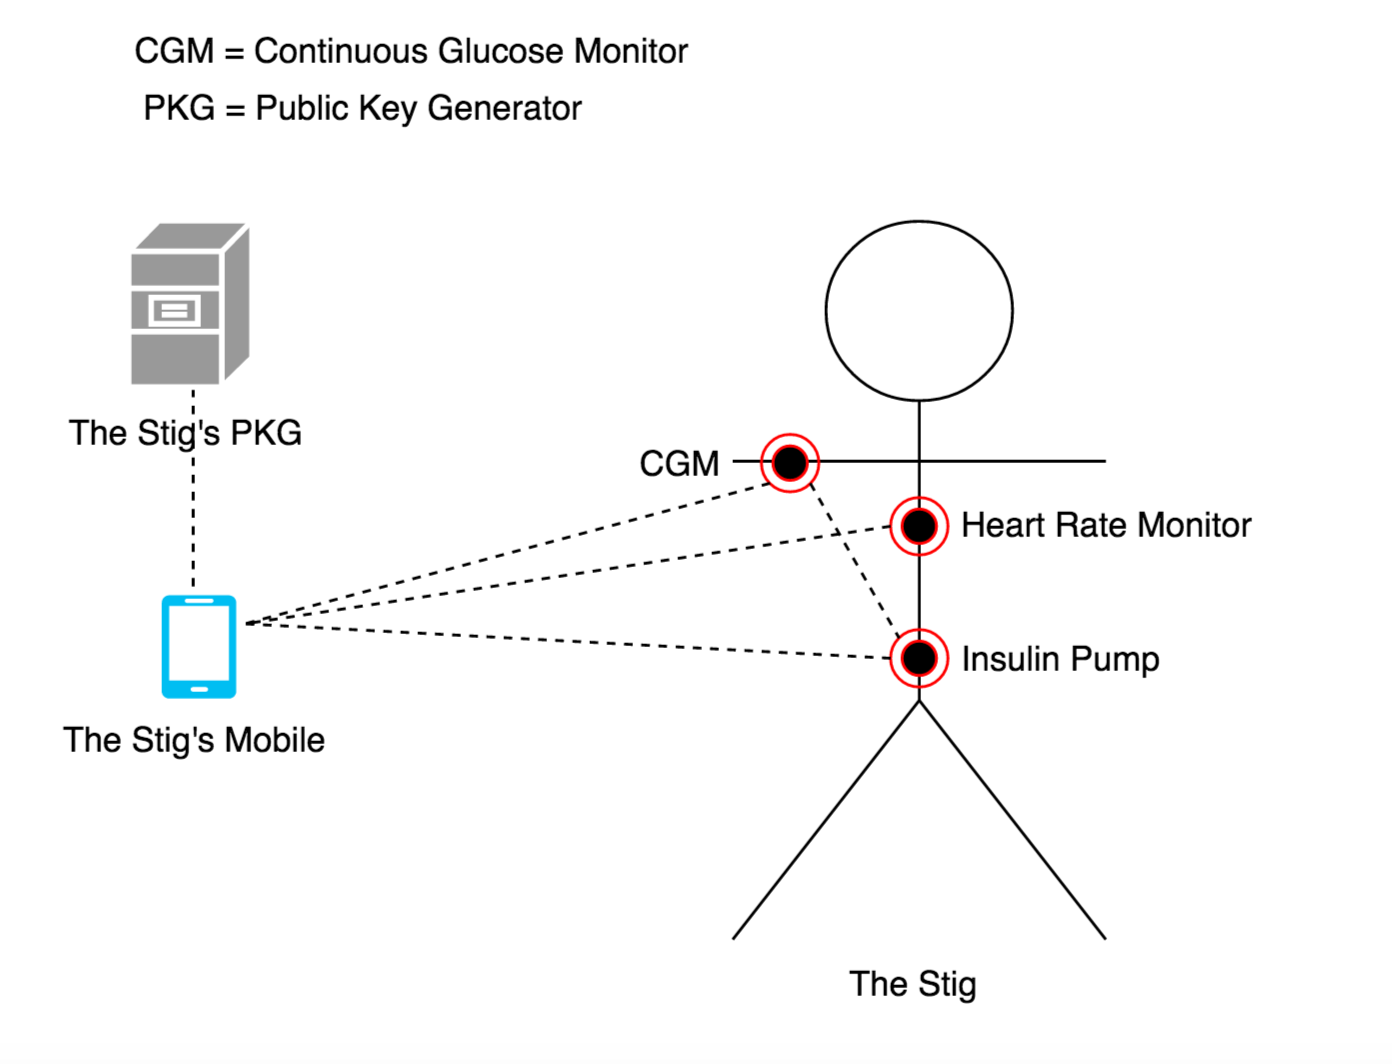
\includegraphics[width=1\textwidth]{health-sensor-system.png}
  \caption{Health Sensor System}
  \label{fig:health-sensor-system}
\end{figure}

\section{Health Sensor System}\label{hss}
To have a secure system, it needs to be established trust between the sensors and the devices.
There need to be integrity controls, confidentiality protection and access control. 
In the following sections, I will describe the protocols suggested for achieving the mentioned goals.

\subsection{Rendezvous Authentication}\label{rendezvous_authentication}
One of the best solutions for authentication of an identity in cryptography is rendezvous authentication, the concept of meeting face-to-face for authenticating who you are talking to. 
In \gls{IoT}, we have in most cases the advantage of identifying devices in a physical matter.
This means that it is possible to authenticate devices, such as sensors. 
Typically, this kind of authentication will rely on 1) manually inspection and 2) digital connection, e.g. through \gls{NFC}.
In the proposed system, I assume that this type of authentication is achieved in a secure matter and do not discuss whether how this should be done.

Also there is the concept of human-computer authentication~\cite{DBLP:journals/iacr/GilbertRS05, DBLP:conf/crypto/JuelsW05, DBLP:conf/percom/Weis05}.
This authentication method uses a shared secret before authentication. 

\subsection{Initialization}\label{init}
The goal for the initialization protocol is to achieve a secure one-round secret key exchange.
For the protocol to be secure, there are several issues that need to be addressed. 
The response message containing the secret key has to be 1) encrypted. 
This can be achieved by using asymmetric encryption on a \gls{CEK} from which is used to do symmetric encryption on the secret key.
The response message has to be 2) signed by the \gls{PKG} for integrity and authenticity reasons.
For it to make sense applying 3) a nonce for replay protection, the communication between the device and the \gls{PKG} has to be unique of some kind.
This implies that the device has to authenticate itself in a way that an adversary cannot do, e.g. a shared secret.
This secret can for instance be a hardware implemented secret in the device that the user reads (from the package) and authenticates manually at the \gls{PKG} before the initialization.
% This leads to 4) mutual authentication. 

When The Stig is setting up his \gls{HSS}, first he wants to configure the \gls{PKG}. 
Any type of computer can play the role of the \gls{PKG} and The Stig has chosen his home server, from now ``the PKG''.
The \gls{PKG} creates two key pairs that is used to do \gls{IBE} and \gls{IBS}.
Second, he wants his mobile device, from now ``the mobile'', to be a part of the \gls{PKG}s trust domain, and further add all of the other devices and sensors, from now ``device(s)''.

In~\autoref{fig:init_ibe_1} the device plays the role as the mobile. 
The \gls{ID} of every device is a part of the Name under which the device registers a prefix.
I.e. a device register \path{/ndn/no/ntnu/<device>/<resource>} and hence its \gls{ID} is \path{/ndn/no/ntnu/<device>}.
To be able to communicate securely under initialization, the device have to create a temporary \gls{MPK} and \gls{MSK} and then extract a temporary secret key for its \gls{ID}. 
At first, the device has to act as a \gls{PKG} for itself to ensure confidentiality, and the trust between the device and the real \gls{PKG} is based on the concept explained in~\autoref{rendezvous_authentication}.
The device sends an Interest appending the temporary \gls{MPK} and the \gls{ID} to the \gls{PKG} asking to join the \gls{PKG}s domain.
The \gls{PKG} encrypts a \gls{CEK} with the temporary \gls{MPK} and the \gls{ID} received from the device. 
Then the \gls{PKG} extracts the secret key for the device (this will be the key belonging to the \gls{PKG}s trust domain) and uses the \gls{CEK} to do a symmetric \gls{AES} encryption on the secret key. 
The Data packet response to the initialization Interest will contain the identity-based encrypted \gls{CEK}, the symmetric encrypted secret key and the \gls{PKG}s \gls{MPK}.
To finish the initialization protocol, the device decrypts the \gls{CEK}, throws away the temporary keys, and finally decrypts the secret key.
The device has established a trust with its \gls{PKG} and can verify other devices in this domain. 

\begin{figure}[ht]
  \centering
  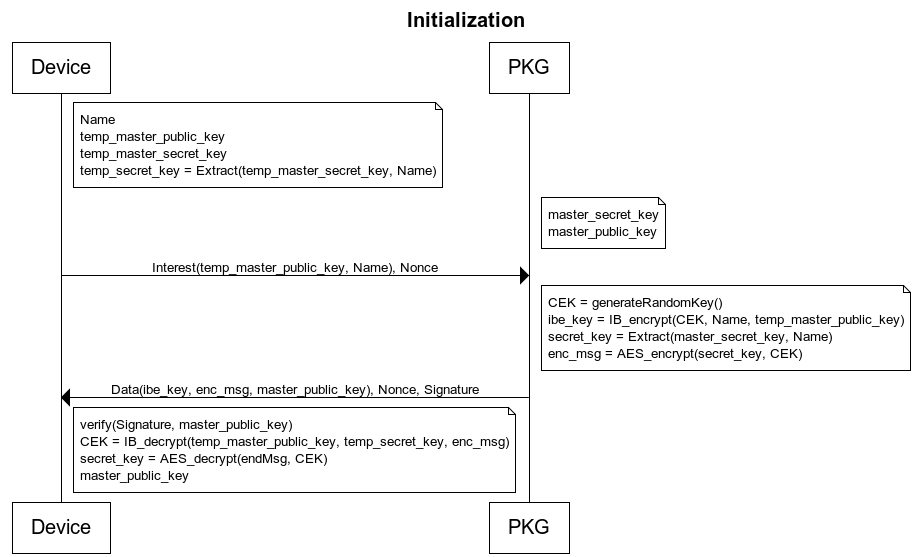
\includegraphics[width=1\textwidth]{Initialization.png}
  \caption{Initialization IBE}
  \label{fig:init_ibe_1}
\end{figure}

Now that the mobile is authenticated, devices can connect to the mobile through e.g. \gls{NFC} for initialization.
This results in a rendezvous authentication between the device and the mobile, and if the mobile is given the authorities to perform initialization (\autoref{access_control}), the new device has joined the \gls{PKG}s trust domain.

\todo{prove secureness of initialization protocol}


% \begin{figure}[ht]
%   \centering
%   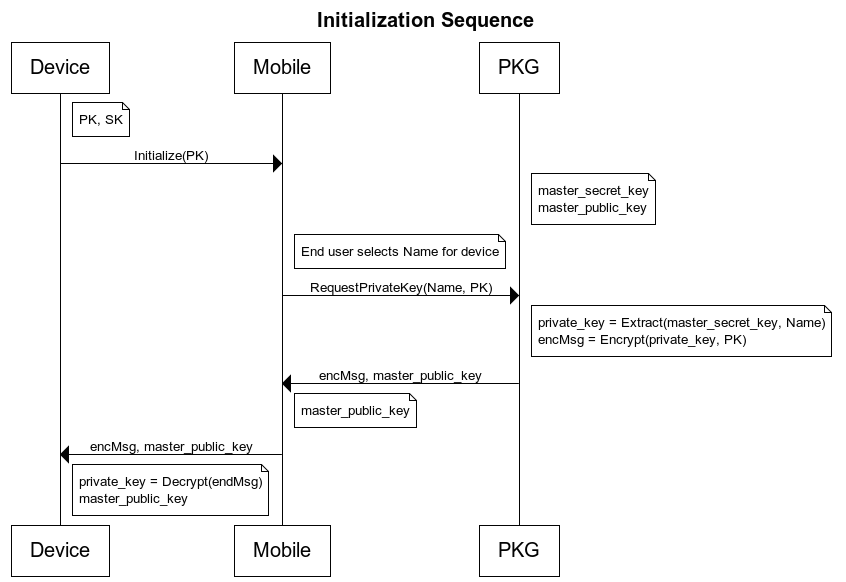
\includegraphics[width=1\textwidth]{init_ibe_2.png}
%   \caption{Initialization IBE through authorized device}
%   \label{fig:init_ibe_2}
% \end{figure}

% \begin{lstlisting}[language=BASH, caption={Initialization}, label={lst:ibe-initialization}]
% pkg = new PublicKeyGenerator;
% for device in {devices}
% do
% 	device -> connect to pkg;
% 	pkg -> verify device then issue secret key;
% 	device -> subscribe Name Sync and Public Key
% done
% \end{lstlisting}

\subsection{Data Pull}\label{data_pull}
The goal for this protocol is to achieve a secure one-round data pull with authorization and integrity.
For the protocol to work and the data pull to be successful, 1) both devices belongs to the same trust domain (i.e. has initialized with the same \gls{PKG}) and 2) the requester has to have granted access rights for the resource requested.

As illustrated in~\autoref{fig:health-sensor-system}, the device has joined the \gls{PKG}s trust domain and are ready to communicate with other devices.
This flow is illustrated in~\autoref{fig:data_pull_ibe}.
First the requester has to express an Interest to the target device asking for a specific resource. 
The requester signs the Interest and appends it to the Content Name.
The receiver checks whether the requester has access rights to the requested resource and verifies that the requester is a part of the same trust domain.
If the requester is authorized, the receiver responds with the Data containing the resource. 
The receiver will also do a symmetric encryption on the sensor data and do a asymmetric encryption on the \gls{CEK} with the requester's \gls{ID}.
This step is only performed if the data confidentiality is needed. 
Then the Data packet is signed and sent.
Finally the requester receives the Data and verifies the signature and decrypts the sensor data.

\begin{figure}[ht]
  \centering
  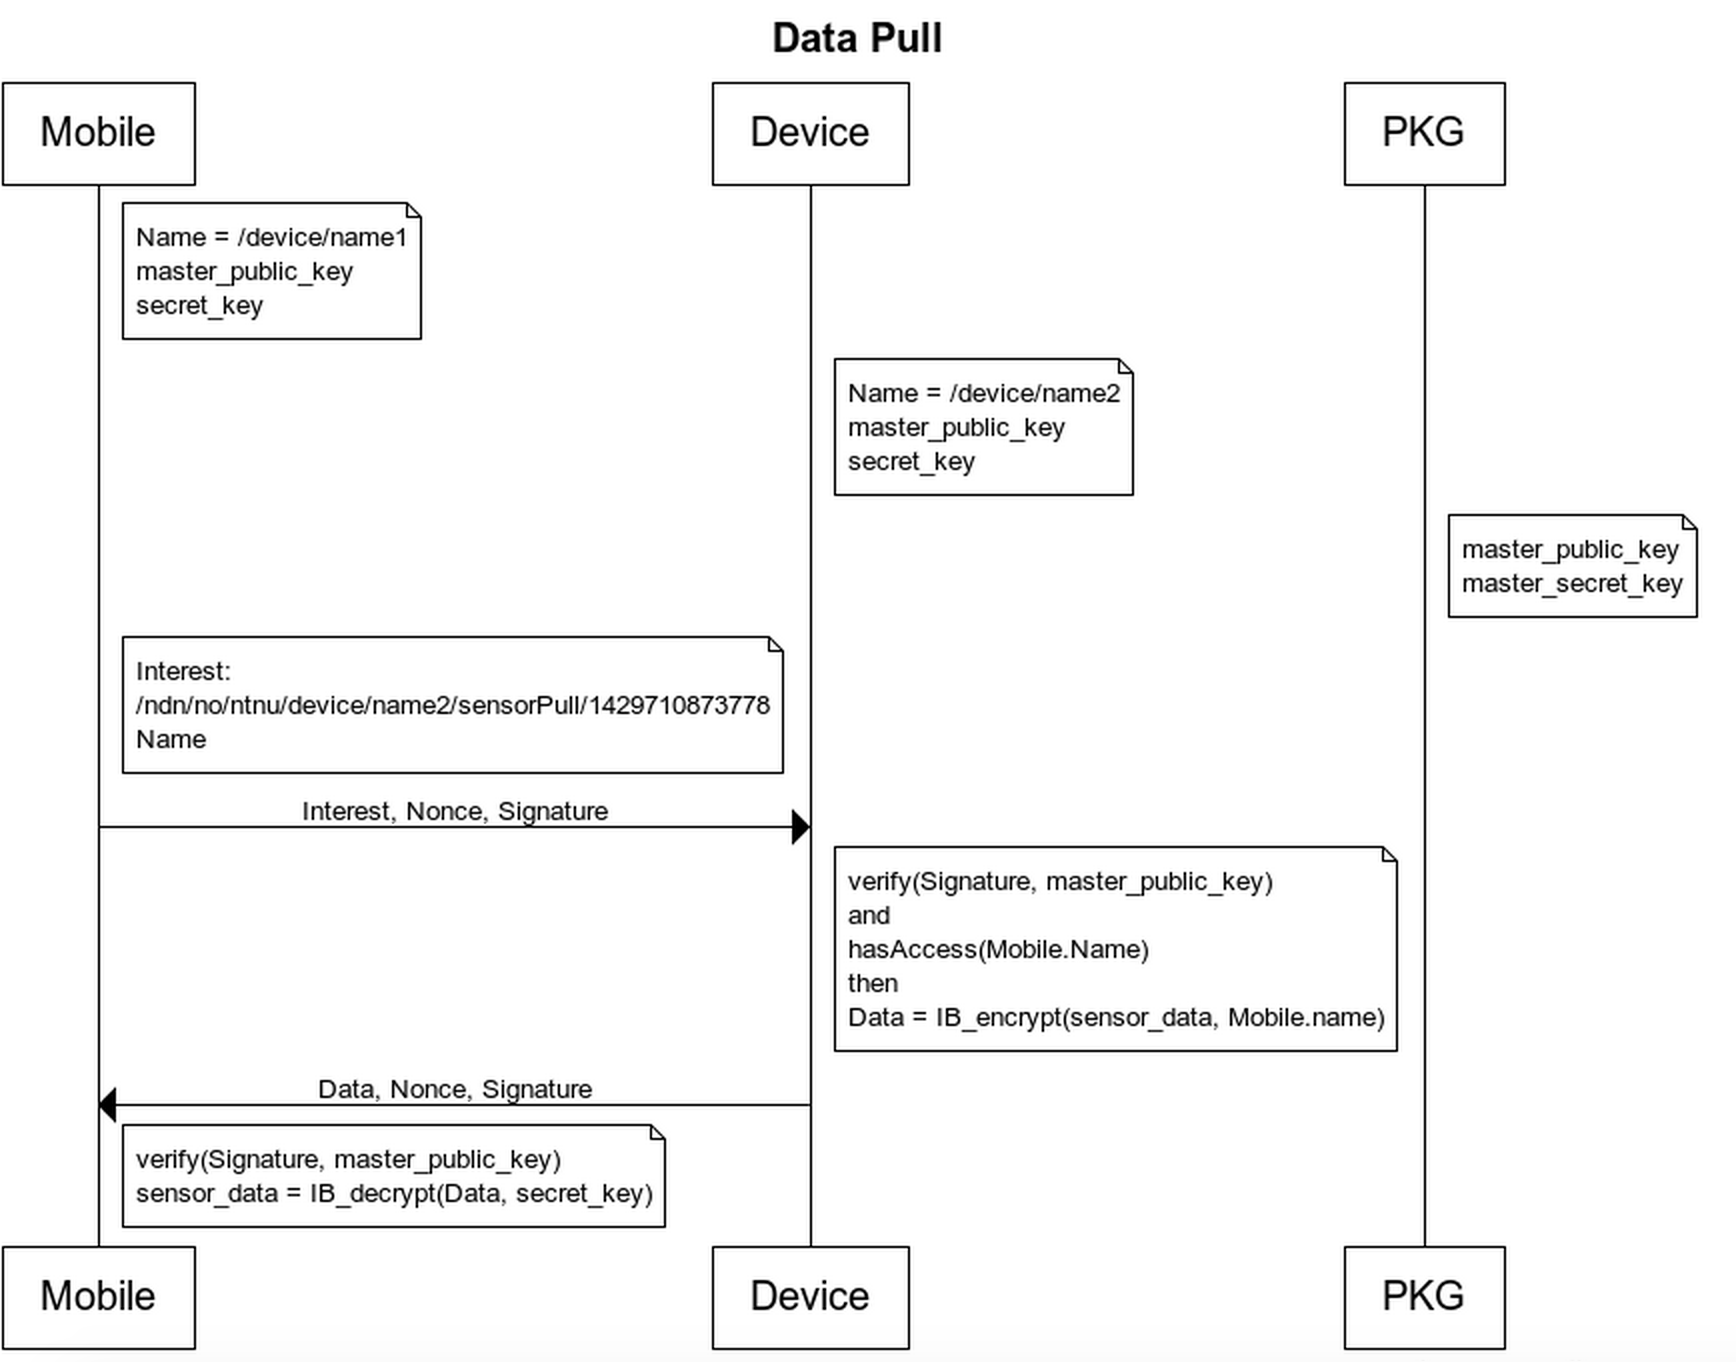
\includegraphics[width=1\textwidth]{DataPull.png}
  \caption{Mobile performing a data pull from a device in the network.}
  \label{fig:data_pull_ibe}
\end{figure}

\todo{prove secureness of data pull protocol}

\subsection{Distribution using File Synchronization Module}

The Stig wants to have full control over the devices that are a part of the trust domain, and be able to remove a device if necessary.
Each device should have an updated list of all public keys, i.e. every devices' \gls{ID}.
The distribution of this list can easily be achieved by using the \gls{FSM} (\autoref{file-sync}).
The \gls{PKG} will be the distributor in this synchronization and each device will be a subscriber.


\section{Trust Model}
In this section the trust model will be explained. 

\subsection{Access Control}\label{access_control}
Since the ID\textsubscript{device} is appended to the Interest and the Interest is signed by the corresponding SK\textsubscript{device}, the \gls{ID} of the device can easily be authenticated. 
since 
When a device retrieves an Interest for its sensor data, there should be an authorization mechanism. 
One solution for this is the Capability Based Approach to \gls{IoT} Access Control~\cite{DBLP:conf/imis/GusmeroliPR12}.
This design has some additional benefits for the \gls{HSS}, such as

\begin{itemize}
  \item delegation support - 
  A device can grant access rights to other devices, as well as granting the right to further delegate these rights to a third device.
  \item capability revocation - 
  If the \gls{PKG} have granted delegation rights to a mobile, and the mobile is not found trustworthy after a while, the capabilities issued by the mobile can easily be revoked.
  \item information granularity - 
  Specific resources from a device can be granted access to in different granularity.
\end{itemize}

One can argue that once a device has been authenticated in the \gls{PKG}s trust domain, everyone in the domain can be sure that the device will not abuse the information or functionalities available. 
However, due to scalability this is not a secure way to handle access control. 
If a device does not need a privilege, it does not need it.
Hence it should not have it. 
That is the least privilege access principle, which is default in~\cite{DBLP:conf/imis/GusmeroliPR12}.

Another solution is to go for a \gls{ACL} based approach equivalent to what they did in~\cite{DBLP:journals/network/ShangDMBZ14}.

\section{Confidentiality, Integrity and Availability}

\begin{description}
  \item[Confidentiality] 
  The encryption can be achieved by encrypting with the Name of the requester.
  As explained in the sequence diagrams presented in the above sections, each Interest appends the requesters Name, hence all packets can be encrypted, and thus the confidentiality in the system is achieved.
  \item[Integrity and Authenticity]
  Each device will obtain a secret key allocated by its superior \gls{PKG}, as explained in~\autoref{ibc}.
  With the concept from~\autoref{rendezvous_authentication} together with the \gls{PKG}s \gls{MPK}, you can trust that the device is authorized for the \gls{PKG}s trust domain. Hence all signed packets can be verified by anyone with the \gls{MPK}.
  Every Interest has a timestamp attached to the Name (e.g. \path{/ndn/no/ntnu/device/name2/sensorPull/1429710873778}), i.e. milliseconds from \texttt{UTC 1970-01-01 00:00:00}, that is used for protection against replay attack. 
  \item[Availability]
  This is a harder problem to solve.
  The network is purely wireless, hence vulnerable to jamming. 
\end{description}